\section{Antecedentes}
\label{section:antecedentes}

Durante décadas, la forma de hacer que un procesador fuera más rápido era aumentar su frecuencia de reloj \cite{sutter2005free}. Sin embargo, al rededor del 2005, los fabricantes se toparon con el \quotes{muro de potencia} (\emph{power wall}), el cual se refiere a la incapacidad de seguir aumentando la frecuencia de reloj de los procesadores sin que el consumo de energía y la generación de calor se vuelvan intratables \cite{hennessy2017computer}. En este sentido, la transición hacia arquitecturas de computación paralela ha sido una necesidad física debido al estancamiento de la escalada de la frecuencia de reloj de los procesadores, en lo que respecta de la Ley de Moore \cite{wazir2019performance}. Véase la figura \ref{fig:moore_stagnation}.

\begin{figure}[h!]
  \centering
  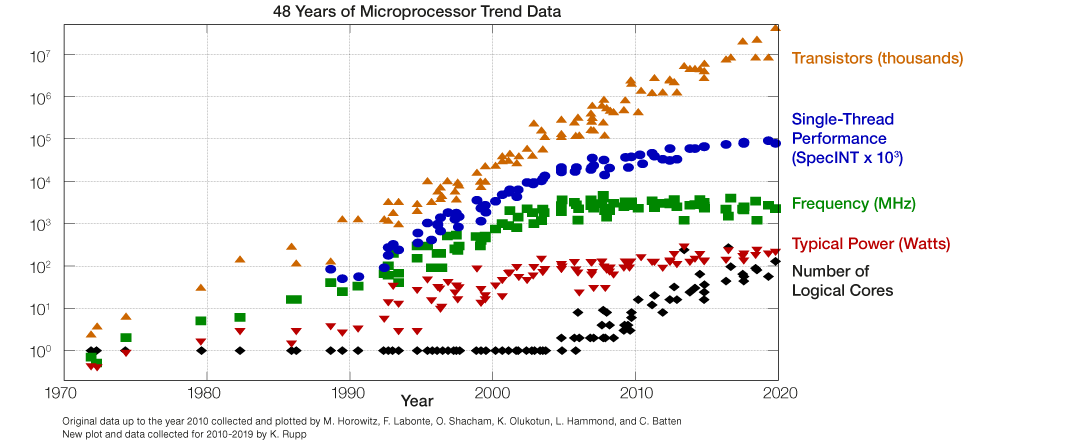
\includegraphics[width=0.65\textwidth]{1-Preliminary/figs/Moores-Law.png}
  \caption{Evolución de la Ley de Moore a través de los años (Tomada de \parencite{man2021stagnation}).}
  \label{fig:moore_stagnation}
\end{figure}

Actualmente, existen diversos trabajos orientados a la implementación paralela de distintas aplicaciones a través de clústeres de bajo costo. Algunos ejemplos son:

\begin{itemize}
  \item \textbf{Trabajo de Cruz Salazar y Fiestas:} en este trabajo se realiza la implementación de un clúster de computadoras para dotar de una máquina de alto rendimiento al CTIC UNI, usando como base computadoras personales recicladas. En este clúster, se realizan pruebas de rendimiento a través del cálculo de PI y simulaciones de N-cuerpos, con el fin de comparar el rendimiento con una computadora moderna \cite{cruz2011construccion}.
  \item \textbf{Clúster hecho con Raspberry Pi:} en este proyecto se crea un clúster de computadoras con las Raspberry Pi, el cual funciona similiar a las supercomputadoras actuales y tiene la finalidad de funcionar como un clúster pequeño y económico en el que los estudiantes e investigadores puedan obtener experiencia práctica. Se realizan programas paralelos y secuenciales para la simulación de Monte Carlo para hallar el valor de PI y un generador de números primos, con el propósito de comparar el tiempo que tardan en ejecutarse en el clúster en paralelo, y en secuencial en una computadora moderna \cite{wazir2019performance}.
\end{itemize}

Con base en lo anterior, se puede ver que la contrucción de arquitecturas paralelas utilizando componentes de bajo costo es una estrategia viable para la realización de herramientas de cómputo de alto rendimiento. Por lo tanto, se propone abordar este paradigma desde un enfoque de viabilidad educativa y sustentabilidad tecnológica, utilizando la paralelización del Juego de la Vida como caso de estudio principal.